% Template for PLoS
% Version 3.3 June 2016
%
% % % % % % % % % % % % % % % % % % % % % %
%
% -- IMPORTANT NOTE
%
% This template contains comments intended 
% to minimize problems and delays during our production 
% process. Please follow the template instructions
% whenever possible.
%
% % % % % % % % % % % % % % % % % % % % % % % 
%
% Once your paper is accepted for publication, 
% PLEASE REMOVE ALL TRACKED CHANGES in this file 
% and leave only the final text of your manuscript. 
% PLOS recommends the use of latexdiff to track changes during review, as this will help to maintain a clean tex file.
% Visit https://www.ctan.org/pkg/latexdiff?lang=en for info or contact us at latex@plos.org.
%
%
% There are no restrictions on package use within the LaTeX files except that 
% no packages listed in the template may be deleted.
%
% Please do not include colors or graphics in the text.
%
% The manuscript LaTeX source should be contained within a single file (do not use \input, \externaldocument, or similar commands).
%
% % % % % % % % % % % % % % % % % % % % % % %
%
% -- FIGURES AND TABLES
%
% Please include tables/figure captions directly after the paragraph where they are first cited in the text.
%
% DO NOT INCLUDE GRAPHICS IN YOUR MANUSCRIPT
% - Figures should be uploaded separately from your manuscript file. 
% - Figures generated using LaTeX should be extracted and removed from the PDF before submission. 
% - Figures containing multiple panels/subfigures must be combined into one image file before submission.
% For figure citations, please use "Fig" instead of "Figure".
% See http://journals.plos.org/plosone/s/figures for PLOS figure guidelines.
%
% Tables should be cell-based and may not contain:
% - spacing/line breaks within cells to alter layout or alignment
% - do not nest tabular environments (no tabular environments within tabular environments)
% - no graphics or colored text (cell background color/shading OK)
% See http://journals.plos.org/plosone/s/tables for table guidelines.
%
% For tables that exceed the width of the text column, use the adjustwidth environment as illustrated in the example
% table in text below.
%
% % % % % % % % % % % % % % % % % % % % % % % %
%
% -- EQUATIONS, MATH SYMBOLS, SUBSCRIPTS, AND SUPERSCRIPTS
%
% IMPORTANT
%
% Below are a few tips to help format your equations and other special characters according to our specifications. For
% more tips to help reduce the possibility of formatting errors during conversion, please see our LaTeX guidelines at
% http://journals.plos.org/plosone/s/latex
%
% For inline equations, please be sure to include all portions of an equation in the math environment.  For example,
% x$^2$ is incorrect; this should be formatted as $x^2$ (or $\mathrm{x}^2$ if the romanized font is desired).
%
% Do not include text that is not math in the math environment. For example, CO2 should be written as
% CO\textsubscript{2} instead of CO$_2$.
%
% Please add line breaks to long display equations when possible in order to fit size of the column.
%
% For inline equations, please do not include punctuation (commas, etc) within the math environment unless this is part
% of the equation.
%
% When adding superscript or subscripts outside of brackets/braces, please group using {}.  For example, change
% "[U(D,E,\gamma)]^2" to "{[U(D,E,\gamma)]}^2".
%
% Do not use \cal for caligraphic font.  Instead, use \mathcal{}
%
% % % % % % % % % % % % % % % % % % % % % % % % 
%
% Please contact latex@plos.org with any questions.
%
% % % % % % % % % % % % % % % % % % % % % % % %

\documentclass[10pt,letterpaper]{article}
\usepackage[top=0.85in,left=2.75in,footskip=0.75in]{geometry}

% amsmath and amssymb packages, useful for mathematical formulas and symbols
\usepackage{amsmath,amssymb}

% Use adjustwidth environment to exceed column width (see example table in text)
\usepackage{changepage}

% Use Unicode characters when possible
\usepackage[utf8]{inputenc}

% textcomp package and marvosym package for additional characters
\usepackage{textcomp,marvosym}

% cite package, to clean up citations in the main text. Do not remove.
\usepackage{cite}

% Use nameref to cite supporting information files (see Supporting Information section for more info)
\usepackage{nameref,hyperref}

% line numbers
\usepackage[right]{lineno}

% ligatures disabled
\usepackage{microtype}
\DisableLigatures[f]{encoding = *, family = * }

% color can be used to apply background shading to table cells only
\usepackage[table]{xcolor}

% array package and thick rules for tables
\usepackage{array}

% create "+" rule type for thick vertical lines
\newcolumntype{+}{!{\vrule width 2pt}}

% create \thickcline for thick horizontal lines of variable length
\newlength\savedwidth
\newcommand\thickcline[1]{%
  \noalign{\global\savedwidth\arrayrulewidth\global\arrayrulewidth 2pt}%
  \cline{#1}%
  \noalign{\vskip\arrayrulewidth}%
  \noalign{\global\arrayrulewidth\savedwidth}%
}

% \thickhline command for thick horizontal lines that span the table
\newcommand\thickhline{\noalign{\global\savedwidth\arrayrulewidth\global\arrayrulewidth 2pt}%
\hline
\noalign{\global\arrayrulewidth\savedwidth}}


% Remove comment for double spacing
%\usepackage{setspace} 
%\doublespacing

% Text layout
\raggedright
\setlength{\parindent}{0.5cm}
\textwidth 5.25in 
\textheight 8.75in

% Bold the 'Figure #' in the caption and separate it from the title/caption with a period
% Captions will be left justified
\usepackage[aboveskip=1pt,labelfont=bf,labelsep=period,justification=raggedright,singlelinecheck=off]{caption}
\renewcommand{\figurename}{Fig}

% Use the PLoS provided BiBTeX style
\bibliographystyle{plos2015}

% Remove brackets from numbering in List of References
\makeatletter
\renewcommand{\@biblabel}[1]{\quad#1.}
\makeatother

% Leave date blank
\date{}

% Header and Footer with logo
\usepackage{lastpage,fancyhdr,graphicx}
\usepackage{epstopdf}
\pagestyle{myheadings}
\pagestyle{fancy}
\fancyhf{}
\setlength{\headheight}{27.023pt}
\lhead{
\includegraphics[width=2.0in]{PLOS-submission.eps}}
\rfoot{\thepage/\pageref{LastPage}}
\renewcommand{\footrule}{\hrule height 2pt \vspace{2mm}}
\fancyheadoffset[L]{2.25in}
\fancyfootoffset[L]{2.25in}
\lfoot{\sf PLOS}

%% Include all macros below

\newcommand{\cursedforest}{\textsc{CursedForest}\xspace}
\newcommand{\ranger}{\textsc{Ranger}\xspace}
\newcommand{\randomforest}{\textsc{randomForest}\xspace}
\newcommand{\mtry}{\texttt{mtry}\xspace}
\newcommand{\ntree}{\texttt{ntree}\xspace}

%% END MACROS SECTION

%% Additional packages
\usepackage{footmisc}
\usepackage{multirow}
\usepackage[T1]{fontenc}
%% required the installation of cm-super 55MB - TeX font package (full version) with CM (EC) in Type1 in T1, T2*, TS1, X2 enc

%%local edits (rob)
\let\oldmarginpar\marginpar
\renewcommand\marginpar[1]{\-\oldmarginpar[\raggedleft\footnotesize #1]%hv
{\raggedright\footnotesize #1}}
\reversemarginpar
\setlength{\marginparwidth}{5cm}
\usepackage{caption}
\usepackage{subcaption}
\usepackage{placeins}
\usepackage{xspace} % see http://tex.stackexchange.com/questions/31091/space-after-latex-commands

\begin{document}
\vspace*{0.2in}

% Title must be 250 characters or less.
\begin{flushleft}
{\Large
\textbf\newline{\cursedforest - A Random Forest Implementation for ``Big'' and ``Wide'' Data} % Please use "title case" (capitalize all terms in the title except conjunctions, prepositions, and articles).
}
\newline
% Insert author names, affiliations and corresponding author email (do not include titles, positions, or degrees).
\\
Aidan O'Brien\textsuperscript{1},
Piotr Szul\textsuperscript{2},
Robert Dunne\textsuperscript{3}, 
Paul Leo \textsuperscript{4},
Emma L. Duncan \textsuperscript{4,5,6},
Stephanie Li\textsuperscript{7},
James Doecke\textsuperscript{7},
Nick Ellis\textsuperscript{8}, and
Denis C. Bauer\textsuperscript{1,*}
%, with the Lorem Ipsum Consortium\textsuperscript{\textpilcrow}
\\
\bigskip
\textbf{1} Health \& Biosecurity, CSIRO, Sydney, NSW, Australia
\\
\textbf{2} Data61, CSIRO, Brisbane, QLD, Australia
\\
\textbf{3} Data61, CSIRO, Sydney, NSW, Australia
\\
\textbf{4} Institute of Health and Biomedical Innovation, Queensland University of Technology, Brisbane, QLD, Australia
\\
\textbf{5} Department of Endocrinology, Royal Brisbane and Women's Hospital, Brisbane, QLD, Australia
\\
\textbf{6} Faculty of Medicine and Biomedical Sciences, University of Queensland, Brisbane, QLD, Australia
\\
\textbf{7} Health \& Biosecurity, CSIRO, Brisbane, QLD, Australia
\\
\textbf{8} Oceans \& Atmosphere, CSIRO, Brisbane, QLD, Australia
\bigskip

% Insert additional author notes using the symbols described below. Insert symbol callouts after author names as necessary.
% 
% Remove or comment out the author notes below if they aren't used.
%
% Primary Equal Contribution Note
%\Yinyang These authors contributed equally to this work.

% Additional Equal Contribution Note
% Also use this double-dagger symbol for special authorship notes, such as senior authorship.
%\ddag These authors also contributed equally to this work.

% Current address notes
%\textcurrency a Insert current address of first author with an address update
% \textcurrency b Insert current address of second author with an address update
% \textcurrency c Insert current address of third author with an address update

% Deceased author note
%\dag Deceased

% Group/Consortium Author Note
%\textpilcrow Membership list can be found in the Acknowledgments section.

% Use the asterisk to denote corresponding authorship and provide email address in note below.
* Denis.Bauer@CSIRO.au
\end{flushleft}

\tableofcontents
\clearpage

% Please keep the abstract below 300 words
\section{Abstract}
We introduce \cursedforest, an implementation of random forests designed to handle data that may have an extremely large
number of variables. We discuss the utility of random forests for machine learning problems. We show on simulated and
real data that the novel implementation can achieve reasonable prediction accuracy and variable importance estimates
even in setting where other implementations, including some designed for large data, fail.

\linenumbers

\section{Introduction}
The digital revolution is seeing a dramatic increase in data collected about almost every aspect of
life~\cite{Loebbecke2015}.  These data sets are not only growing vertically, by capturing more events, but also
horizontally by capturing more information about these events.  The challenge of big and ``wide'' data is especially
pronounced in the health space where, for example, whole genome sequencing (WGS) technology enables researchers to
interrogate all 3 billion base pairs of the human genome.

Identifying the relevant or disease specific base-pair difference between individuals is the focus of genome wide
association studies (GWAs).  These analysis are typically performed on only the most frequently differing base-pairs,
termed single nucleotide polymorphisms (SNPs), by applying linear or logistic regression analysis to each SNP
separately~\cite{CCC2007}.  It has since been demonstrated that not taking interactions between SNPs into account
when filtering for potential disease mutations is inadequate~\cite{Manolio2009,Yang2011}.

A tree based model is capable of taking the interaction of variables into account \cite{Wright.et.al.2016}. In addition, random forests are well
suited for processing ``wide'' genomic data for two reasons.  Firstly, while other machine learning applications have
the propensity to overfit datasets with more features $p$ than samples $n$ (a consequence of the ``curse of
dimensionality''~\cite{Bauer2014, bellman1961adaptive}), decision trees are resistant to overfitting.  Secondly, random
forests are also very easy to parallelize. As the forest is a sum of decision trees, it is possible to grow separate
trees on different processors and combine the trees. See the discussion of the properties of random forests in Section
\ref{section:methods}.

The most popular random forest software packages are R-based, although current implementations do not scale well with
increasing feature size~\cite{Wright.and.Ziegle.2016}.  This is despite R now supporting long vectors (length greater
than $2^{31}-1$), and the \randomforest implementation in R lending itself to parallelization to grow multiple
trees simultaneously~\cite{Liaw.and.Weiner.2002} and them combine them.  More suitable implementations for ``wide''
genomic data have been developed in other programming languages. \textsc{CloudForest} \cite{Bressler2015} written in Go,
achieves fast run times by effective use of the CPU cache, optimizing for different classes of features and efficiently
multi-threading.  Similarly, \ranger~\cite{Wright.and.Ziegle.2016} written in C++ with an R front-end is
specifically optimized for dealing with large data sets.

The use of traditional compute infrastructure limits the parallelization strategies that can be employed by  
these methods.  The programs are limited to utilizing only CPUs that are on the same computer node (multi-threading) or
else they run on CPUs distributed across nodes by virtue of the fact that there is no communication between the
processes (a separate tree is grown on each node).  Hadoop/Spark overcomes these limitation by enabling programs to
scale beyond compute-node boundaries and hence enable more sophisticated parallelization strategies.  In the case of
random forests this means that the computations for each node of a tree can be handed off to separate processors.
  
Here we introduce \cursedforest, a Hadoop/Spark based implementation of random forests specifically designed to cater
for ``big'' (many samples) and ``wide'' (many features) data sets. A Spark application runs on a ``driver'' node and
distributes tasks to many ``worker'' nodes, or ``executors''. Using this facility, \cursedforest is capable of
parallelization the split for each node in a tree thereby handling millions of features. It can, for example, fit a
model to the 1000 Genomes Project data, which consists of approximately 2500 samples with up to 80 million
variants~\cite{1KG2012}.  By also utilizing Spark to read in and manipulate the standard genomic variant format (VCF)
directly, \cursedforest outperforms existing tools even on small datasets where multi-threading generally performs
well. Harnessing the virtually unlimited capability to parallelize tasks, \cursedforest can build a large number of
trees and use a high \mtry value which may lead to greater accuracy (see the example in section \ref{section:synthetic}). 

\marginpar{does \cite{Szymczak2016} say that high \ntree gives greater  accuracy for variable importance selection?
Check this. }

We previously demonstrated the versatility and scalability of Spark by developing VariantSpark~\cite{OBrien2015}, a
framework allowing users to easily analyze Variant Call Format (VCF) files using ML algorithms on the Spark framework.
Using VariantSpark, we successfully built a k-means model on the full $2500 \times 80$ million matrix to cluster
individuals by their ethnicity achieving an Adjusted Rand Index (ARI) of 0.84 (with 1 being perfect clustering and -1
random clustering).

Here we extend this toolkit to encompass supervised learning using random forests.  Spark ML's random forest
implementation is not able to handle the extremely ``wide'' genomic data as it was developed for large number of samples
with only modest dimensionality.  Although Spark ML can build a random forest model on a subset of the data (chromosome
1), the time taken is excessive due to the large amount of data being aggregated and processed by the driver node during
intermediate stages of building the model (see Table~\ref{timingtable}).  This unbalanced work load where the driver
node becomes the bottleneck and worker nodes being idle prevents a seamless scaling to larger datasets. The memory
requirements per executor also increases with dimensionality due to the data types Spark ML uses, which we elaborate on
in the discussion.

\cursedforest is included in our previously developed framework for Spark-based genomic data analysis,
VariantSpark~\cite{OBrien2015}, which therefore now enables supervised and unsupervised machine learning. This offers a
comprehensive analysis toolkit that can scale for the future data demands, where the richness from WGS data can be
utilized to ``fill in'' or impute the information at previously unobserved genomic positions in older array
technology~\cite{Howie2012}.  This provides the potential to impute samples in the GWAs catalogue and generate datasets
of hundreds of thousands of individuals with millions of variants, highlighting the need for incorporating modern
compute paradigms to deal with these challenges.

In the first section we explore some of the properties of random forests as these will also be apparent in the
\cursedforest implementation. Here we provide demonstrations using synthetic data.  We then demonstrate the scalability
of \cursedforest in respect to the dimensionality of the data, building a random forest model on whole-genome data from
the 1000 Genomes Project. We report the error in predicting ethnicity.  Finally, given the role
different parameter values can play in model construction, we explore the effect tuning these parameters can have on the
prediction accuracy of the model.



\section{Methods}
\label{section:methods}

%%%%%%%%%%%%%%%%%%%%%%%%%%%%%%%%%%%%%%%%%%%%
\subsection{Overview of Random Forests}

Decision trees have a number of desirable features, they:
\begin{itemize}
  \item are invariant to monotonic scaling of the data;
  \item can handle categorical and real valued inputs;
  \item can handle missing values;
  \item are insensitive to uninformative predictors;
  \item are able to capture interactions between features (which is of importance for modelling complex polygenic diseases).
  \end{itemize}
However, the tree fitting algorithm is greedy and may generate an unstable model. That is, a small change in the data may
lead to a very different model. 

Random forests apply the technique of bootstrap aggregation or bagging to decision trees.  The training data sets are
independently drawn, with replacement, from the joint distribution of $(X,Y)$ so that each set comprises $n$
$(p+1)$-tuples $(x_1,y_1),\ldots, (x_n,y_n)$. This is done $B$ times and a tree is grown on each of these $B$ samples.
The results are then combined in an appropriate way. In a classification problem we take the majority vote for the trees
over the $q=1,..,Q$ classes,
\begin{equation*}
{{h_f}}= \arg \max_q \left(\sum_b I(h(x;B_b)=q)\right).
\end{equation*}
In addition to growing the trees
on bootstrapped samples, each node in the tree is split on a randomly
selected subset of the variables.

Random forests are a variance reduction technique. They take unpruned tree models, which have a low bias but a high
variance, and by combining them reduce the variance.  For regression problems, as the prediction error is the sum of the
variance and the bias squared, this strategy should lead to a low prediction error.

For classifiction problems there is no obvious decomposition of classification error into an equivalent bias plus
variance form. A number of different additive decompositions of classification error have been considered in an effort
to understand the success of bagging. They are all less transparent than the regression case (see \cite{Friedman.1997} and
citations therein).

In the case of a regression tree, the average prediction error for an individual tree $h(X; B)$ is
\begin{equation}
PE_t = E_B E_{X,Y} (Y-h(X; B))^2.
\end{equation}
Assume that, for all $B$, the tree is unbiased, i.e., $EY= E_X h(X; B)$. Then
\begin{equation}
PE_f \leq \rho PE_t
\end{equation}
where $\rho$ is the weighted correlation between residuals $(Y-h(X;B))$ and $(Y-h(X;B^\prime))$ for independent
$B,B^\prime$.
So what is required for accurate random forest regression is (i) low correlation between residuals of differing tree in
the forest, and (ii) low prediction error for the individual trees \cite{Segal.2004}. 

The benefits of random forest models are:
\begin{itemize}
\item they give an out-of-bag (OOB) estimate of model accuracy, by using the samples not selected for the bootstrapped sample
  as an independent test set for each tree;
\item they provide a measure of variable importance, for example by summing the number of times a variable is used to
  split a node, over all nodes and all trees. More complex measures of variable importance are also used;
\item they inherit some of the qualities of tree models (but not, for example, the handling of missing values via surrogate
  variables. This would be difficult as the trees are split on random subsets of variables).
\end{itemize}

Since the original implementation of random forests, there have been a number of developments leading to a better
understanding of the algorithm.
\begin{itemize}
\item random forests are resistant to overfitting. However it is not true that they will not overfit,
  ~\cite{Segal.2004} gives examples of overfitting in cases where:
  \begin{itemize}
  \item a single tree is the most appropriate model; and
  \item the variables are highly correlated so that the bootstrap resampling does not give rise to uncorrelated trees.
  \end{itemize}
However, keeping these difficult cases in mind, random forests have a strong claim to being resistant to overfitting.
\item \cite{Strobl.et.al.2007} demonstrates that the random forest algorithm is subject to a bias in variable selection
  via two mechanisms:
  \begin{enumerate}
  \item differences in variable scale (for $X_i$ continuous) and number of levels (for $X_i$ discrete) introduces a
    bias. An uninformative variable with a large number of levels may be selected over a more informative variable with
    fewer levels;
  \item bagging introduces a bias, but sampling $(1- 1/e) \approx 0.632$ of the data without replacement seems to be an
    effective strategy for removing the problem.
  \end{enumerate}
\end{itemize} 

\cite{Strobl.et.al.2007} introduce changes to the random forest algorithm to fix 1) and 2).  Effect 1) will be apparent
in the \cursedforest algorithm as well.  However, there are many examples, particularly in genomics, where we have data
sets that are:
\begin{itemize}
\item very wide;
\item all variables have the same number of levels (for example, measurements at different points along the genome);
\item the hypothesized functional relationship is of a form amenable to a decision tree.
\end{itemize}
GWAs data sets are an obvious application areas for this algorithm. 

\cite{Biau.2012} provides a proof that a random forest model will converge at a rate that depends on
the cardinality of the set $S$ of ``strong predictors'' rather than on the number of variables $p$. That is, given a
function $y=f(S)$ depending on a set of variables $S$, a random forest will converge to the true function $y$ with a
rate that depends on the size of $S$ and not the number of noise variables in the data set. If the size of $S$ is small
compared to the total number of variables, then the rate of convergence will be quicker. It is not clear what the size
of the set $S$ will be in a GWAs application. There are cases of small groups of SNPs with large effects and also of
conditions caused by the interaction of large groups of SNPs.

\cite{Genuer.et.al.2010} and \cite{Diaz.and.Alvarez.2006} describe iterative schemes for doing variable selection using
the importance measure. See \cite{Chen.and.Ishwaran.2012} for a review of the area with particular reference to genomic
data.

%%%%%%%%%%%%%%%%%%%%%%%%%%%%%%%%%%%%%%%%%%%%%%%%%%%%%%%%%%%
\subsection{\cursedforest}
VariantSpark made use of Spark's machine learning algorithms ``Spark ML''. While Spark ML algorithms demonstrate
scalability when dealing with a large number of samples, this scalability eventually breaks down as we include more
features.

As is standard with Spark applications, we store our data in a Resilient Distributed Dataset (RDD), where an RDD is
essentially a collection of elements. In the case of Spark ML, each element in the RDD is a sample. RDDs contribute to
the scalability of Spark as they can distributed across multiple nodes and operated on in parallel. Even as we add more
samples to a dataset, Spark can simply schedule extra tasks to handle the additional items in the RDD.

However, within an RDD, spark ML stores each sample as a vector. Unlike RDDs, which can be partitioned and distributed
across multiple nodes, each vector must be present in its entirety on any node accessing it. This is no problem with
typical datasets, however as dimensionality increases, the vectors eventually reach a size where they can no longer fit
into a single node's memory.

So in the case of adding more samples, Spark ML can simply create more tasks, keeping memory consumption within the
cluster's bounds. However, as the dimensionality of each sample grows, the memory requirements of the job increases to
enable these increasingly large vectors to be loaded into memory.  

On the other hand, \cursedforest is specifically designed to handle wide ``cursed'' data. It avoids the relation between
memory and dimensionality by avoiding calculations that rely on entire feature vectors and taking the parallelization
work down to the level of the individual features.  For each node of a tree, \cursedforest will distribute
tasks that consist of single features (variants), for every individual.  Each of these tasks will calculate the
information gain for that specific feature.  Once these tasks have completed, the results are reduced to return the
feature which gives the greatest information gain.  This process is then repeated until \cursedforest has created the
entire decision tree.

The current implementation of \cursedforest uses a ``Gini impurity'' criteria for splitting. Let $f_q$ be the fraction
of items labelled with value $q$ where $q = 1, \ldots, Q$ at a node. The Gini impurity is
$$
I_G(f) = \sum_{q = 1}^Q f_q ( 1 - f_q ), 
$$
which is a minimum when all observations at the node are in the same class.

%%%%%%%%%%%%%%%%%%%%%%%%%%%%%%%%
% This section talks about the datasets
%%%%%%%%%%%%%%%%%%%%%%%%%%%%%%%%
\subsection{Datasets}
\subsubsection{1000 Genomes Project}
We obtained the 1000 Genomes Project data as VCF files from their FTP site.  Each VCF file contains the variants for
every individual across one chromosome.  We use the phase 3 dataset which contains 2,504 individuals with approximately
81 million variant positions (i.e. a matrix of $2,504 \times 81$ million).  For compatibility with the majority of the
algorithms we demonstrate, we convert the original variant representations to double representations.  For example, we
store the absence of a variant (0\textbar0) as 0, a heterozygous
variant (1\textbar0 or 0\textbar1) as 1, and a
homozygous variant (1\textbar1) as 2.  However, this is not the only possible encoding \cite{Goldstein.et.al.2011}. Note that from
the encodings listed in Table~\ref{table:encodings}, the additive encoding will present the most difficulty for a random
forest model.


\begin{table}[!ht]
%\begin{adjustwidth}{-2.25in}{0in} % Comment out/remove adjustwidth environment if table fits in text column.
\begin{flushleft} 
\centering
\caption{\bf Possible encodings of GWAS data \cite{Goldstein.et.al.2011}}
\begin{tabular}{|l|l|l|l||}
\hline
{\bf Type} & {\bf Mechanism}                                         & {\bf Partition} \\ 
\thickhline
Additive   & Each additional minor allele increases variation        & 0, 1, 2         \\
Dominant   & Presence of at least 1 minor allele increases variation & 0, 1/2          \\
Recessive  & Two minor alleles needed for variation                  & 0/1, 2          \\
Heterosis  & Heterozygote leads to variation                         & 0/2, 1          \\ \hline
%\end{adjustwidth}
\end{tabular}
\label{table:encodings}
\end{flushleft}
\end{table}


\subsubsection{Bone mineral density dataset}
We obtained a VCF file from the authors of \cite{Duncan.2011}, which contains variant data from 1,936 postmenopausal women.
This dataset covers approximately 7 million variant positions. We have information about the bone mineral density (BMD)
for each individual, where a low BMD is a major predisposing factor to fracture \cite{Duncan.2011}. 

\subsubsection{Synthetic data} 
\label{section:synthetic_data}
 Each dataset consists of $n$ samples and $p$ variables where $n << p$,
and values for each variable are ordinal variables with three levels represented as numbers $\{0, 1, 2\}$ (which
correspond to an additive effect encoding of genomics variation) randomly generated from uniform distribution with equal
probabilities.  

The model paramters are $w_i = 1/\sqrt{2^{i-1}}$ for $i =1,\ldots 5$ and we set 
$$
z =  \sum_{i=1}^{i=5} {w_i x_i}.
$$
We let $\sigma_\epsilon^2 = Var(z)(1- 0.125)/0.125 $ and then 
$y =   z + \epsilon$ where $\epsilon \sim  N(0, \sigma_\epsilon^2).$
The dichotomous response is generated by thresholding $y$ at the $0.8$ quantile.



\subsection{Parameter settings}
We consider the parameter setting for the random forest algorithm. We use the R notation from the \randomforest
package \cite{Liaw.and.Weiner.2002} which incorporates the original Fortran code by Brieman and Cutler.  We incorporate
the advice of \cite{Liaw.and.Weiner.2002}, which we have found mirrors our own experience:
\begin{itemize}
\item \ntree{}  -- the number of trees.  The number of trees necessary for good performance grows with the number of
  predictors.  \cite{Liaw.and.Weiner.2002} suggest that a high \ntree is necessary to get stable estimates of variable
  importance and proximity; however, even though the variable importance measures may vary from run to run, we note that
  it is possible for a random forest model to have a poorer fit and still have an accurate ranking of variable
  importance;
\item \mtry{}  -- the number of variables considered at each split (if \mtry=$p$, we have a boosted decision
  tree model).  If one has a very large number of variables but expects only very few to be ``important'', using larger \mtry may give
  better performance;
\item the size and complexity of the individual trees is controlled in \randomforest by setting \texttt{nodesize}, the
  minimum size of terminal nodes. It is controlled in Spark ML by setting \texttt{maxDepth}, the maximum depth of each
  tree in the forest\footnote{The Spark ML documentation \cite{Spark.2016} sets \texttt{maxDepth} to 4 in their
    classification example. This may give an estimate with a higher bias and, as such, may be a poor choice. See the
    discussion in \cite{Dietterich.2002} where it is shown that bagging may reduce bias as well as variance but gives a
    better result for low bias learners. \cite{Dietterich.2002} notes that if the bootstrap replicate approximation were
    correct (i.e.~if the bootstrap sample came from an identical distribution to the data), then bagging would reduce
    variance without changing bias.} In the TCGA example the RandomForests code produced trees with depths of 30+.
\end{itemize}



%%%%%%%%%%%%%%%%%%%%%%%%%%%%%%%%
%
% Results
%
%%%%%%%%%%%%%%%%%%%%%%%%%%%%%%%%
\section{Results and Discussion}



%%%%%%%%%%%%%%%%%%%%%%%%%%%%%%%%
% Section 1:  Feature Selection and classification on synthetic data
%%%%%%%%%%%%%%%%%%%%%%%%%%%%%%%%
\subsection{\cursedforest can evaluate variable importance for millions of features}
\label{section:synthetic}
In this section we demonstrate the two features of \cursedforest, namely variable importance analysis to select the most
associated set of features amongst millions of dimensions as well as its ability to accurately classify the labels of
high-dimensional samples.  We therefore generate a synthetic dataset with 2.5 million variables (features, p) of which 5 
are the response variable and 5000 samples (n), as discussed in the methods section.

We fit the random forest model to obtain the classification accuracy by capturing the out-of-bag error (OOB) and perform the variable importance analysis where we expect to retrieve the
5 features in order of the weight that was assigned to them, which is captured by the rank-biased-overlap (RBO) \cite{Webber2010} measure.
We are running Apache Spark 1.6.1 on a YARN cluster with 12 worker nodes each with 16 Intel Xeon E5-2660@2.20GHz CPU cores and 128 GB of RAM.

%mtry = number of variable seclection at each node - proportion of p 
%ntree= number of trees 

% mtry large makes trees correlated because the same important features have a higher chance of being selected
% overfitting because it picks random that happen to be 

As shown in Fig~\ref{figure:out-of-bag-prediction-error-prod.png} the default value for \mtry (number of variables selected at each node) does not result in a 
good classification performance for this large feature dataset. Note, that the plot shows the proportion of $n/p$ for \mtry\ with the default being $\sqrt{p} \approx 1581$. 
The OOB  for this value of \mtry does not exceed 0.5 on a scale from 0 (perfect) to 1 (random), even when the number of trees are increased (\ntree). 

Increasing \mtry\ in combination with \ntree\ yields best performance with the OOB error essentially constant around 0.4 across a large range of 
of \mtry and \ntree values. 
This is in contrast to the feature-selection performance, where the RBO measure heavily depends on \ntree\ and gives better results with lower values of \mtry, where 
the best RBO is around 0.85 on a scale from 0 (no feature recovered) to 1 (fully recovered).

This may be because a large \mtry\ generates more correlated trees as the same important features have a higher chance of being selected in all, not yielding good performance outcomes. 
This issue is less pronounced for classification tasks where random features can mimic the response variable, hence resulting more in a performance plateau. 
Increasing the number of trees on the other hand improves performance especially when 
the trees are kept diverse (small \mtry) but appropriate for large feature datasets (\mtry larger than default). \cursedforest's feature of parallelising trees at the node level hence cater perfectly for the 
requirement of large feature datasets as more trees can be built given a fixed time budget. 

%Fig~\ref{figure:synth1} illustrates the effect of varying \mtry and \ntree on these two measures. The default \mtry
%value for a classification problem is $\sqrt{p} \approx 1581$ so in this case we are considering values considerably larger than
%the default. Fig~\ref{figure:out-of-bag-prediction-error-prod.png} shows the OOB error is constant across a large range of 
%of \mtry and \ntree values whereas Fig~\ref{figure:rbo-prod.png} illustrates that the RBO measure depends
%heavily on \ntree but gives a better value with lower values of \mtry.

From the synthetic data we can conclude that \cursedforest is able to perform accurate feature selection as well as
accurate classification for large numbers of samples with large feature vectors.
We can also conclude that fine tuning the model to accurately classify the dataset does not ensure good feature selection performance as there seems to be little correspondence between the OOB and RBO measure.



\begin{figure}[tbhp] 
  \begin{adjustwidth}{-1.00in}{0in}
    \caption{\textbf{Out of bag classification error and rank-biased-overlap estimates}} 
    \label{figure:synth1}
    \begin{subfigure}[b]{0.5\linewidth}
      \centering
      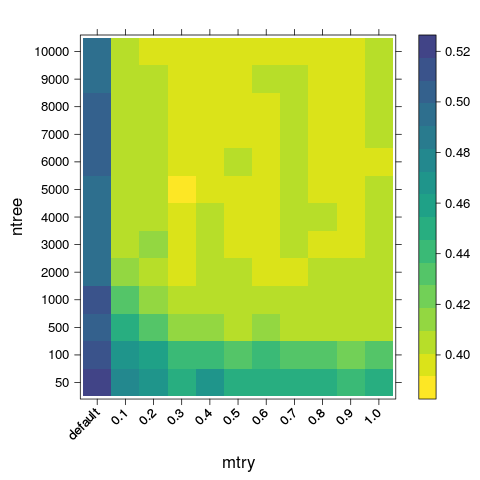
\includegraphics[totalheight=8cm]{./figs/oob_levleplot.png}
      \caption{OOB classification error.} 
      \label{figure:out-of-bag-prediction-error-prod.png} 
      \vspace{4ex}
    \end{subfigure} 
    \begin{subfigure}[b]{0.5\linewidth}
      \centering
      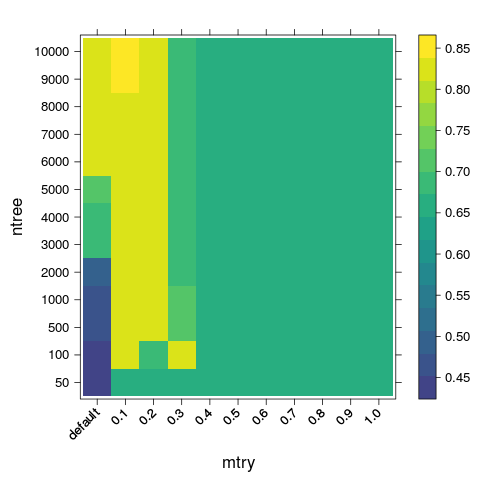
\includegraphics[totalheight=8cm]{./figs/rbo_levleplot.png}
      \caption{The rank-biased-overlap measure.} 
      \label{figure:rbo-prod.png} 
      \vspace{4ex}
    \end{subfigure} 
    \begin{flushleft} 
      Random forests with 100 trees were trained on the synthetic dataset of 2.5M features and 5K samples.
      Each measure is shown as a function of \mtry and \ntree. Note that the plot colors have been chosen so that the lighter color indicates
      the better result, that is, a lower OOB or a higher RBO.
    \end{flushleft}
  \end{adjustwidth}
\end{figure}

%%%%%%%%%%%%%%%%%%%%%%%%%%%%%%%%
% Section 2: Feature Selection on real data 
%%%%%%%%%%%%%%%%%%%%%%%%%%%%%%%%
\subsection{\cursedforest\ selects previously demonstrated bone-density variants}
In this section we use \cursedforest\ to identify genomic locations that are associated with a specific trait. To do this, we perform feature selection over XX genomic variants to 
identify the locations associated with Bone Mineral Density (BMD)~\cite{Duncan.2011}. We build a
model on the BMD dataset (see datasets) using a binary high or low BMD value as the label.  From this model, we output a
list of the top 10,000 contributing variants, ranked by their Gini impurity. The variant with the highest Gini impurity,
and hence importance, is ranked 1, and the variant with the lowest Gini impurity is ranked 10,000.  

%DENIS: number
To test whether the associated features have biological meaning, we investigate whether the known BMD genes investigated by Duncan {\it et al.}~\cite{Duncan.2011} are enriched amongst the 
highly ranked genes. We therefore label all variants that fall within XXbp of these 32 BMD genes and observe that they are
ranked significantly higher than other locations in the genome (Mann-Whitney U, $p=1.3\times10^{-07}$), supporting our hypothesis that biologically relevant features are contributing more information to our classification model.

We therefore investigate the highest-ranked features not amongst the associated gene list by Duncan {\it et al.}~\cite{Duncan.2011}. 
%DENIS is this correct about the transcription factor binding site?
COLEC10 (collectin 10) contains variants more recently associated with BDM~\cite{Kemp2014,Liu2008}, with a verified transcription factor binding site for the known BMD gene FOXL1.
%However, we also observe that from the set of highest-ranked features, for example, the top ten, not all of them exist
%within close proximity to known BMD genes. We investigate the literature to determine the plausibility of these variants
%contributing to BMD.
%One gene is COLEC10 (collectin 10). Featuring a transcription factor binding site for FOXL1, COLEC10 is also reported as
%containing variants associated with BMD \cite{Kemp2014,Liu2008}. However there currently exists no information on how this gene
%may contribute to BMD. 
Also highly-ranked are variants in chromosome 22q11. Stagi {\it et al.}~\cite{Stagi.2010}, observe that individuals with a
microdeletion in this region have a significant reduction in bone mass. In this same region, we also observe
variants present in PRODH (proline dehydrogenase). PRODH catalyzes the first step in proline degradation, and as
proposed by Phang {\it et al.}~\cite{Phang.2008}, proline is made available by collagen degradation.

Investigating the lowly-ranked genes, we observe DCDC5 (Doublecortin Domain Containing 5) ranked 9,667 out of 10,000. This gene is 
one of the BMD-associated genes postulated by literature that Duncan {\it et al.}~\cite{Duncan.2011} inspect.
Similar to their findings, our results also indicate that this gene does not have a strong association with BMD. 
In fact, DCDC5 is not highly expressed in bone, and any mechanisms by which this gene might regulate BMD are unclear \cite{Thakker2012}. 
Although variants near DCDC5 are associated with BMD \cite{Rivadeneira2009}, it is questionable as to whether the gene itself contributes to BMD.


In Table~\ref{featuretable}, we display the top 10 features, ranked by their Gini impurity measure in the random forest model.

\begin{table}[!ht]
%\begin{adjustwidth}{-2.25in}{0in} % Comment out/remove adjustwidth environment if table fits in text column.
\centering
\caption{
{\bf Features from the TCGA BRCA dataset ranked by their importance.}}
\begin{tabular}{|l|l|l|l|l|l|l|}
\hline
{\bf Variant} & {\bf Gene} & {\bf Importance}\\ \thickhline
x:xxxx & cell2 row 1 & cell3 row 1\\ \hline
x:xxxx & cell2 row 2 & cell3 row 2\\ \hline
x:xxxx & cell2 row 3 & cell3 row 3\\ \hline
\end{tabular}
\begin{flushleft} 
Here the importance is the Gini impurity measure when building a model using the cell type as the label.
\end{flushleft}
\label{featuretable}
%\end{adjustwidth}
\end{table}






%%%%%%%%%%%%%%%%%%%%%%%%%%%%%%%%
% Section 3: Classification selection
%%%%%%%%%%%%%%%%%%%%%%%%%%%%%%%%
\subsection{\cursedforest outperforms existing methods for classification problems}
In this section we compare \cursedforest's performance against other published methods for predicting ethnicity on the
1000 Genomes Project dataset.

In a previous paper, we clustered individuals from the 1000 Genomes Project using k-means clustering \cite{Obrien2016}.
\marginpar{reference is missing}
Although we were able to cluster individuals on all 80 million variants, it was relatively slow, with the entire
process (pre-processing and clustering) taking over 30 hours.
We investigate building random forest models on this data. However, we observed this process to not only be slower
than building a k-means model, but does not scale to as many dimensions (see Table~\ref{timingtable}). To keep
the following comparisons fair, we limit the number of executors available to Spark. On the relatively low-dimensional
phase1\_chr22 dataset (1,092 x 490,036), we observed a runtime of under 8 minutes. Although slower than Ranger, 
presumably due to the overhead of Spark's distributed platform on this relatively small dataset, we observe Spark ML to
be about 16 minutes faster than R. Moving to the larger dataset, phase3\_chr1 (2,504 x 6,450,364), we observe an increase
in Spark ML's runtime to over 8 hours. Moving to our next largest dataset, phase3\_chr1\-3 (2,504 x 19,328,051), and the
job fails to complete within our arbitrary cutoff time of 20 hours.

From our trials, it was apparent that Spark ML, although designed to handle many samples, is unable to efficiently cope
with a huge number of features. With the decreasing costs of genome sequencing, this case will surely become increasingly
common.

\cursedforest solves this problem of high-dimensionality genomic data. Not only is it faster on the above smaller datasets,
but it is also able to scale to the entire genome. In Table~\ref{cursedforesttable} we present our observed times building
models with CursedForest using all available resources on our Spark cluster.

As we previously mentioned, building a random forest model on the phase3\_chr1 dataset with Spark ML takes over 8 hours.
Building a model with \cursedforest, however, takes only 20 minutes using the same cluster setup and this time drops to
nearly 4 minutes using the entire compute cluster. Subsequently, phase3\_chr1\-3 takes about 11 minutes, and building a
model on the entire genome is just shy of 37 minutes. Not only does the job complete successfully, but building a random
forest model on all 22 autosomes (phase3\_chr1\-22) using \cursedforest is more than twice as fast as building a random
forest on the chromosome 1 (phase3\_chr1) using Spark ML.


\begin{table}[!ht]
\begin{minipage}{\textwidth}
\centering
\caption{ {\bf Performance comparison with \cursedforest on different subsets of the 1000 Genomes Project data.}}
\begin{tabular}{| l | r | l |}
\hline
{\bf Genome \%} & {\bf Error} & {\bf Runtime} \\ \thickhline
phase1\_chr22: 1,092 x 490,036 & 0.04 & 1 min 5 seconds \\ \hline
phase3\_chr22: 2,504 x 1,103,548 & 0.06 & 1 min 37 seconds \\ \hline
phase3\_chr1: 2,504 x 6,450,364 & 0.04 & 4 min 10 seconds \\ \hline
phase3\_chr1-3: 2,504 x 19,328,051 & 0.02 & 10 min 49 seconds \\ \hline
phase3\_chr1-22: 2,504 x 81,047,467 & 0.01 & 36 min 54 seconds \\ \hline
\end{tabular}
\begin{flushleft} 
Comparison of runtime and error for models built using \cursedforest on different subsets of variant data 
from the 1000 Genomes Project.
Each random forest model consists of 50 trees and was built using 130 worker nodes, each with 8GB RAM.
\end{flushleft}
\label{cursedforesttable}
\end{minipage}
\end{table}



\begin{figure}[tbhp] 
    \caption{\textbf{Runtime comparison on the 1000 genomes project}} 
    \label{figure:synth1}
      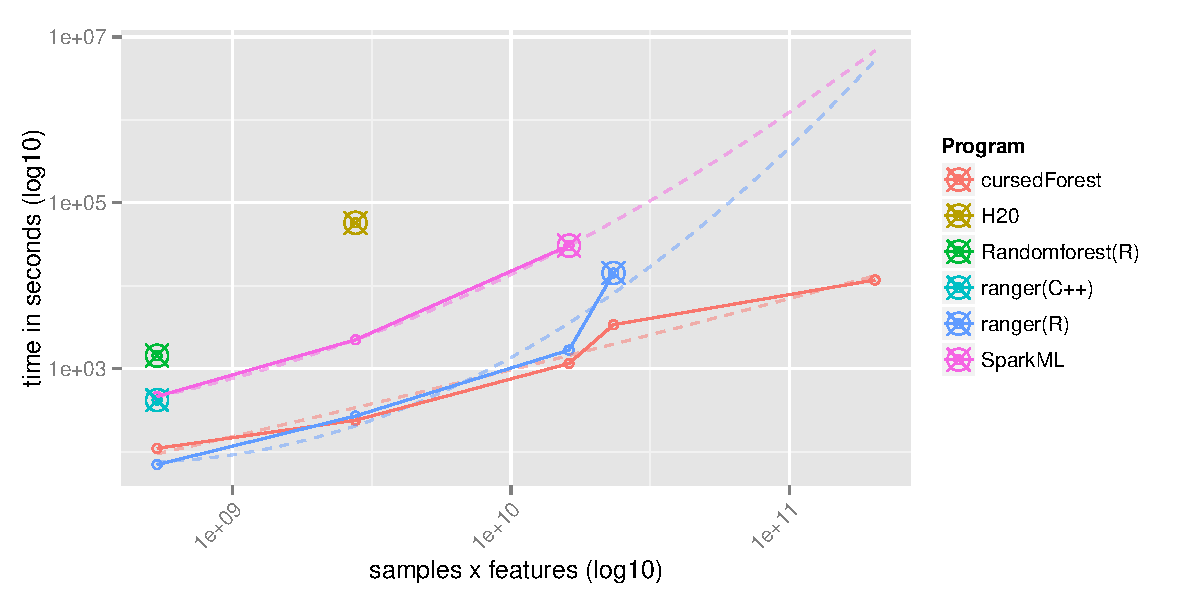
\includegraphics[totalheight=8cm]{./figs/1000genomesRuntime.pdf}
    \begin{flushleft} 
      The figure shows the runtime for the 5 subsets of the 1000 genomes project and the different methods investigated. $\bigotimes$ marks the last dataset the different method completed before running out of memory or running more than 24 hours. The dashed lines mark the trajectory for how ranger and Spark ML had performed given larger memory machines. 
    \end{flushleft}
\end{figure}


\iffalse

\begin{table}[!ht]
\begin{minipage}{\textwidth}
%\begin{adjustwidth}{-2.25in}{0in} % Comment out/remove adjustwidth environment if table fits in text column.
\centering
\caption{ {\bf Performance comparison between the different random forest implementations.}}
\begin{tabular}{| l | l | r | l |}
\hline
\bf{Genome \%}                      & \bf{Method} & \bf{Error}  & \bf{Runtime}  \\

\hline

\multirow{5}{*}{phase1\_chr22: 1,092 x 490,036} & \cursedforest & 0.04  & 1 min 50 seconds    \\ %110
                                                & Spark ML  &  0.05           &           7 min 44 seconds         \\  %464
                                                & \randomforest (R)         & 0.05       & 24 min           \\ %1440
                                                & \ranger (R)      & 0.06       & 1 min 10 seconds       \\ %70
                                                & \ranger (C++)     & 0.06       & 7 min            \\ %420
                                                & H2O           & ??       & ??         \\

\hline

\multirow{5}{*}{phase3\_chr22: 2,504 x 1,103,548}   & \cursedforest & 0.06 & 4 min 2 seconds \\  %240
                                                    & Spark ML  & 0.06 & 37 min 19 seconds \\  %2239
                                                    & \randomforest (R)        & NA         & NA                \\
                                                    & \ranger (R)    & 0.06       & 4 min 30 seconds     \\  %270
                                                    & \ranger (C++)     &     ??   & ??        \\
                                                    & H2O           & 0.05       & 16 hours         \\ %57600

\hline

\multirow{3}{*}{phase3\_chr1: 2,504 x 6,450,364}    & \cursedforest & 0.04  & 19 min 19 seconds         \\ %1159
                                                    & Spark ML  & 0.04       & 8 hour 29 min        \\ % 3403
                                                    & \randomforest (R)        & NA         & NA                \\
                                                    & \ranger (R)      &  0.05       & 28 mins         \\ %1680
                                                    & \ranger (C++)     & ??       & ??            \\
                                                    & H2O           & NA       & NA         \\
\hline

\multirow{3}{*}{phase3\_chr1-3: 2,504 x 19,328,051} & \cursedforest & 0.02  & 56 min 43 seconds             \\ %3403
                                                    & Spark ML &    NA         &   NA               \\ %30540
                                                    & \randomforest (R)        & NA         & NA                \\
                                                    & \ranger (R)      & 0.03      &    3 hour 58 min     \\ %14280
                                                    & \ranger (C++)     & ??       & ??            \\
                                                    & H2O           & NA       & NA         \\
\hline

\multirow{4}{*}{phase3\_chr1-22: 2,504 x 81,047,467} & \cursedforest & 0.01  & 3hour 16min \\ %11760
                                                    & Spark ML & NA & NA  \\
                                                    & \randomforest (R)        & NA         & NA                \\
                                                    & \ranger (R)       &        NA     &        NA    \\
                                                    & \ranger (C++)       &        NA     &        NA    \\
                                                    & H2O           & NA       & NA         \\
\hline




\end{tabular}
\begin{flushleft} 
Comparison of different various machine learning libraries on different subsets of variant data 
from the 1000 Genomes Project.
Each random forest model consists of 50 trees.
\end{flushleft}
\label{timingtable}
%\end{adjustwidth}
\end{minipage}
\end{table}

\fi


%%%%%%%%%%%%%%%%%%%%%%%%%%%%%%%%
% Section 4: Sensitivity 
%%%%%%%%%%%%%%%%%%%%%%%%%%%%%%%%
\subsection{Scalability analysis}
In this section we explore the performance of \cursedforest by testing its ability to scale to different sizes of data
and computational resources.

In order to asses these characteristics we ran \cursedforest classification on synthetic datasets with varying numbers
of variables (features) and samples, similar to the dataset used in \cite{Wright.and.Ziegle.2016} to evaluate
\ranger, allocating varying number of CPU cores to the \cursedforest and also varying the computational complexity
of the random forests by using a range of \mtry values.

We investigate the different synthetic datasets generated for section \ref{section:synthetic_data} and measured the time
taken to build a random forest model of 100 trees. The results reported below are averages of 5 runs, and all the cases
were executed with the same random seed, to improve the consistency of measurements.

First we look at \cursedforest horizontal scalability for a medium size dataset of 2.5 million variables and 5000
samples, by varying the \mtry  fraction and the number of CPU cores allocated to the execution. 
The results are  visualized in Fig~\ref{figure:synthetictiming} below. 
%The raw results are
%presented in Table~\ref{synthetictimingtable} and visualized in figure \ref{figure:synthetictiming} below. 
Regardless of the number of cores used, \cursedforest displays approximately linear dependency between the execution
time and \mtry (Fig~\ref{figure:synthetictiming.a}).

\cursedforest scales almost linearly with the number of CPU cores for medium values of \mtry fraction but for both
lower and higher values the performance degrades slightly (Fig~\ref{figure:synthetictiming.b}). In the latter case the likely cause is
communication overhead (with lower \mtry values the proportion of time for parallelizable computation to the time for
internode communication is lower) while in the latter case it is most likely caused by reaching the clusters
computational capacity.

\marginpar{tables 2 has been commented out -- there is no data in it. Piotr could add the data or we could remove both
  tables just leave the figures. I have done this for the time being} 
Next we investigate \cursedforest scalability with
regards to the size of data, by varying the number of variables and sample for a fixed \mtry fraction of 0.25 and
execution of 128 CPU cores. The results are visualized in Fig~\ref{figure:synth2} below (please note log scale on the
axes and the values on y axes are expressed as trees per hour).

Generally, the number of trees per hour decreases with an increased number of variables and samples sizes. Some
irregularities in the graph can be attributed to computation vs communication tradeoff. It is also worth noting that
keeping the \mtry fraction constant results in higher \mtry values with the growing number of variables, and this is what
drives the performance down rather that the increase of dataset size itself.

To conclude \cursedforest is capable of processing datasets with 50M variables and 10K samples, which is the order of
magnitude of the entire genome variants expected in such dataset, for which it can build approximately 60 trees per
hour.

\begin{figure}[tbhp]
  \begin{adjustwidth}{-1.00in}{0in}
    \caption{\textbf{Scalability of the wide random forest on the synthetic dataset of 2.5M features and 5K samples.}}
    \label{figure:synthetictiming}
    \begin{subfigure}[b]{0.45\linewidth}
      \centering
      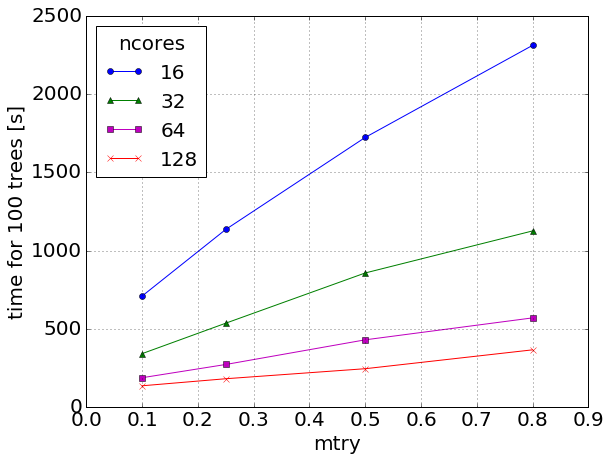
\includegraphics[totalheight=6cm]{./figs/mtry_cpu.png} 
      \caption{Time in seconds to build 100 trees for different \mtry\ fractions. } 
      \label{figure:synthetictiming.a} 
      \vspace{4ex}
    \end{subfigure} 
    \hfill
    \begin{subfigure}[b]{0.45\linewidth}
      \centering
      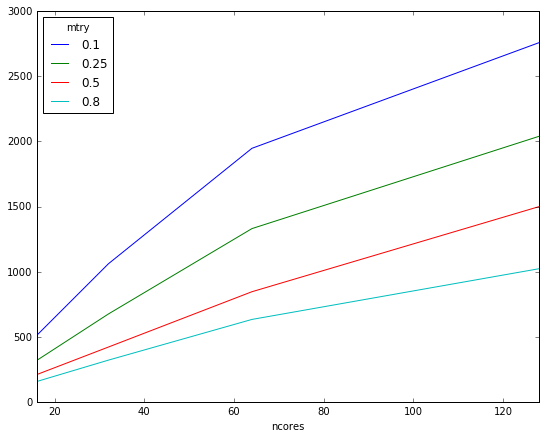
\includegraphics[totalheight=6cm]{./figs/cpu_mtry_trees_per_hour.png}
      \caption{Number of trees build per hour when using a growing number of CPU cores.}
      \label{figure:synthetictiming.b}
      \vspace{4ex}
    \end{subfigure} 
  \end{adjustwidth}
\end{figure}

% commented this table out -- see above
% \begin{table}[!ht]
%   \begin{adjustwidth}{-1.00in}{0in}
%     \centering
%     \caption{\textbf{
%  Time in seconds to build a random forest of 100
%   trees on 128 CPU cores with varying numbers of variables and samples.}}
% \label{synthetictimingtable}
% \begin{tabular}{|l|l|l|l|l|l|l|}
% \hline
% \multicolumn{2}{|l|}{\multirow{2}{*}{}}           & \multicolumn{5}{c|}{Number of variables} \\
% \cline{3-7}
% \multicolumn{2}{|l|}{}                               & \bf{150,000} & \bf{500,000} & \bf{2,500,000}  & \bf{10,000,000} & \bf{50,000,000} \\
% \hline                                                            
% \multirow{4}{*}{Number of samples}      & \bf{1000}  & 21.6  & 26.7  & 59.8  & 133.5  & 668.8 \\
%                                         & \bf{5000}  & 45.7  & 71.9  & 186.2 & 729.3  & 2887.4 \\
%                                         & \bf{10000} & 70.2  & 120.2 & 397.3 & 2237.8 & 5747.8 \\
% \hline
% \end{tabular}
% \end{adjustwidth}
% \end{table}



\begin{figure}[tbhp]
  \begin{adjustwidth}{-1.00in}{0in}
    \caption{\textbf{Scalablity of the Wide Random Forest on synthetic datasets with varying number of samples and variables.}}
    \label{figure:synth2}
    \begin{subfigure}[b]{0.5\linewidth}
      \centering
      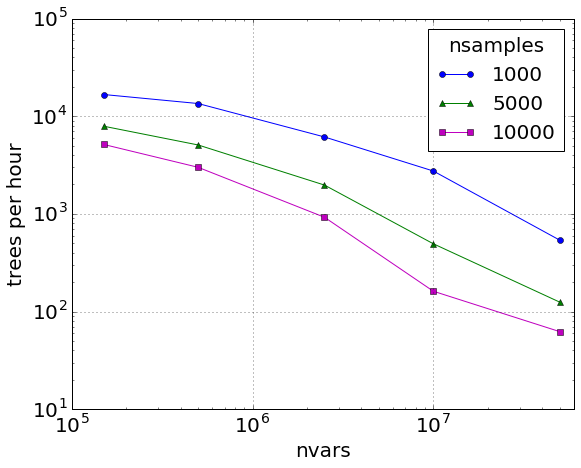
\includegraphics[totalheight=6cm]{./figs/nvars_nsamples.png} 
      \caption{Number of trees build per hour when growing number of variables.} 
      \label{figure:synth2.a} 
      \vspace{4ex}
    \end{subfigure} 
    \begin{subfigure}[b]{0.5\linewidth}
      \centering
      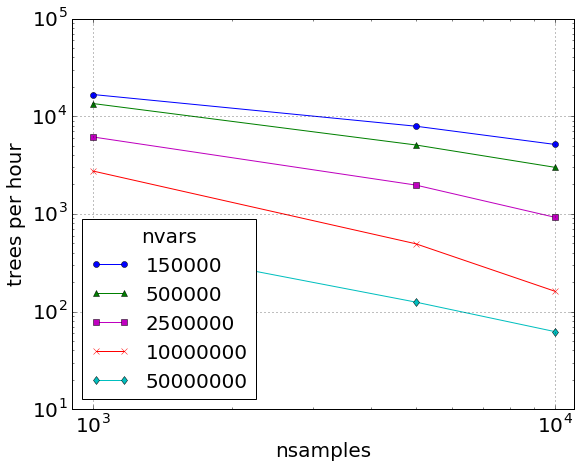
\includegraphics[totalheight=6cm]{./figs/nsamples_nvars.png}
      \caption{Number of trees build per hour when growing number of samples.}
    \label{figure:synth2.b}
    \vspace{4ex}
  \end{subfigure}
\end{adjustwidth}
\end{figure}

% no data in this table 
% \begin{table}[!ht]
% \caption{
% {\bf Sensitivity analysis on parameter choice.}}
% \begin{tabular}{|l|l|l|l|l|l|l|l|}
% \hline
% %\multicolumn{4}{|l|}{\bf Heading1} & \multicolumn{4}{|l|}{\bf Heading2}\\ \hline
% \bf{ \mtry\ }  & \bf{Mtree} & \bf{depth} & \bf{Accuracy} & \bf{Runtime} & \bf{Memory} \\
% \hline
% &&&&&\\ \hline
% \end{tabular}
% \begin{flushleft} 
%   Table notes here.
% \end{flushleft}
% \label{table2}
% \end{table}




\section{Conclusion}
We have demonstrated that using a different parallelization model can extend random forests to the case of an
extremely large number of variables. We have treated the case of variable selection in a $p >> n$ model where most of
the variables are uninformative and have demonstrated the utility of the model for large GWAs data sets. By comparing
this implementation to other implementations (including those optimized for large data sets) we have demonstrated the
utility of this approach.

Donoho and Tanner \cite{Donoho.and.Tanner.2009} give a ``universal phase change'' result that has applications in a
large number of areas including variable selection in high dimensions. Consider
Fig~\ref{figure:phase-diagram-equivalence.png} which shows the region where a model can recover the important variables,
plotted as a function of $\delta = n/p$ and $\rho =k/n$ (where $k$ is the number of significant variables). There is a
distinct boundary, shown empirically and also based on arguments from combinatorial geometry, to the region where we can
reliably recover significant variables.  \cite{Donoho.and.Stodden.2006} investigate the behaviour of a number of
regression approaches for variable selection (LARS, Lasso and forward stepwise) and make the point that above the
phase-transition line variable recovery is still possible by a combinatorial approach.

It is not surprising that that it is more difficult to recover the signal variable in the upper-left area of the figure,
as the problem is both under-determined and sparse. What is surprising is the connection with arguments from
combinatorial geometry. This suggests that we are seeing a universal rule rather than an implementation issue. As
\cursedforest is designed for extremely large numbers of variables it is likely to be operating in difficult regions of
the figure where the ratio $\delta = n/p$ is small.


We note several things here:
\begin{itemize}
\item the Donoho-Tanner phase transition arises in recovering the $\beta$ in data generated by a
  linear model. However, in a decision tree (random forest) there is no notion of estimating the $\beta$
\item A decision tree (random forest) is a heuristic search. It may recover a relationship in the space of the
  combinatorial search.
\end{itemize}

The existence of the  Donoho-Tanner phase transition is a salutary warning. There are likely to be limits, both
computational and logical, to the recovery of signals from noisy data. \cursedforest  is a contribution to addressing the
practical limits but the logical limits will still apply. However in the case of data that is both big and wide,
\cursedforest and other VariantSpark methods may provide a useful tool.


\begin{figure}[tbhp] 
 \begin{adjustwidth}{-1.00in}{0in}
    \caption{\textbf{The Donoho-Tanner phase chage diagram.}}
    \centering
    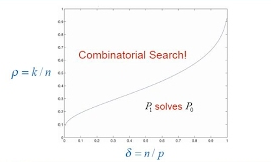
\includegraphics[totalheight=6cm]{./figs/phase.png} 
    \label{figure:phase-diagram-equivalence.png} 
    \vspace{4ex}
  \end{adjustwidth}
\end{figure}


\clearpage
\section{Supporting Information}

% Include only the SI item label in the subsection heading. Use the \nameref{label} command to cite SI items in the text.
%\subsection*{S1 Video}
%\label{S1_Video}
%{\bf Bold the first sentence.}  Maecenas convallis mauris sit amet sem ultrices gravida. Etiam eget sapien nibh. Sed ac ipsum eget %enim egestas ullamcorper nec euismod ligula. Curabitur fringilla pulvinar lectus consectetur pellentesque.


\section*{Acknowledgments}

Cras egestas velit mauris, eu mollis turpis pellentesque sit
amet. Interdum et malesuada fames ac ante ipsum primis in
faucibus. Nam id pretium nisi. Sed ac quam id nisi malesuada
congue. Sed interdum aliquet augue, at pellentesque quam rhoncus
vitae.

\nolinenumbers

\bibliography{CursedForest}

\end{document}

